  \section{Кинематика точки}
  \begin{df}
  Материальная точка - точка, размером которой можно пренебречь.
  \end{df}
  
  \noindent Мы будем полагать, что время меняется равномерно и непрерывно.
  \begin{center}  
  \begin{picture}(100, 100)
  \put(40,40){\vector(1,0){50}} %
  \put(40,40){\vector(0,1){50}} %
  \put(40,40){\vector(-1, -1){25}} %
  \put(40,40){\vector(2,1){40}} %
  \put(92,42){$x$} %
  \put(42,92){$z$} %
  \put(8,8){$y$} %
  \put(82,62){$\v{r}$} %
  \qbezier(50,70)(60,80)(80,60) %
  \qbezier(80,60)(85,50)(90,50) %
  \end{picture}
  \end{center}
  \subsection{Векторное описание движения}
  Зависимость координат от времени назовем законом движения.
  $$ \v{r} = \v{r}(t) \in C^2 $$
  \begin{df}
  $ \gamma = \{ \v{r}(t),~ t \in (0,~ +\infty) \} $ - траектория
  \end{df}
  $$ \v{v} = \frac{d\v{r}}{dt} $$
  $$ \v{w} = \frac{d\v{v}}{dt} = \frac{d^2\v{r}}{dt^2} $$
  \subsection{Декартовы координаты}
  $$ \v{r}(t) = x(t)\v{e_x} + y(t)\v{e_y} + z(t)\v{e_z} $$
  $$ \v{v}(t) = \dot x(t)\v{e_x} + \dot y(t)\v{e_y} + \dot z(t)\v{e_z} $$
  $$ \v{w}(t) = \ddot x(t)\v{e_x} + \ddot y(t)\v{e_y} + \ddot z(t)\v{e_z} $$
  \subsection{Движение по окружности}
  $$ 
  \begin{cases}
   x = R \cos \varphi \\
   y = R \sin \varphi
  \end{cases} 
  $$

  $$ 
  \begin{cases}
  \dot x = -R \sin \varphi \cdot \dot \varphi \\
  \dot y = R \cos \varphi \cdot \dot \varphi 
  \end{cases}
  $$
  
  $$ 
  \begin{cases}
  \ddot x = -R \cos \varphi \cdot  \dot \varphi^2 - R \sin \varphi \cdot \ddot \varphi \\
  \ddot y = -R \sin \varphi \cdot  \dot \varphi^2 + R \cos \varphi \cdot \ddot \varphi 
  \end{cases}
  $$
  
  \begin{center}
  \begin{picture}(100,100)
  \put(50,50){\circle{50}} %
  \put(50,50){\line(1,1){14}} %
  \put(50,50){\line(-1,-1){14}} %
  \put(5,50){\vector(1,0){90}} %
  \put(97,52){$x$} %
  \put(50,5){\vector(0,1){90}} %
  \put(52,97){$y$} %
  \put(65,65){$\varphi(t)$} %
  \put(36,36){\vector(1,-1){10}} %
  \put(40,15){$\v{\tau}$} %
  \put(36,36){\vector(1,1){10}} %
  \put(31,40){$\v{n}$} %
  \end{picture}
  \end{center}
  
  $$ \v{v} = R\dot\varphi(-\sin \varphi \cdot \v{e_x} + \cos \varphi \cdot\v{e_y}) = R \dot\varphi \v{\tau} $$
  $$ \v{w} = R \ddot\varphi ( - \sin \varphi \cdot \v{e_x} + \cos \varphi \cdot \v{e_y}) + R \dot\varphi^2(-\cos \varphi \cdot \v{e_x} - \sin \varphi \cdot {\v{e_y}}) = R \ddot \varphi \v{\tau} + R \dot \varphi^2 \v{n}  $$
  
  $$ \v{v} = R \dot\varphi \v{\tau} = v \v{\tau}$$
  $$ \v{w} = R \ddot\varphi \v{\tau} + R \dot \varphi^2 \v{n} = \dot v \v{\tau} + \frac{v^2}{R} \v{n}$$
  
  \subsection{Естественное описание движения}
  Кривая задана параметрически естественным параметром $s$. $ ds = |\v{dr}| \neq 0 $
  \begin{df}
  \begin{equation} 
  \label{tang}
  \v{\tau} = \frac{d\v{r}}{ds} = \vec r' \text{ - касательный вектор}
  \end{equation}
  \begin{equation}
  \label{normal}
  \v{n} = \frac{\vec \tau'}{|\vec {\tau}'|} \text{ - вектор главной нормали }
  \end{equation}
  \begin{equation}    
  \v{b} = [\v{\tau}; \v{n}] \text{ - вектор бинормали }
  \end{equation}  
  \end{df}
  
  \begin{ass} 
  $ \{\v{\tau}, \v{n}, \v{b}\} $ - тройка ортогональных единичных векторов.
  \end{ass}
  \begin{proof}  
  \begin{flalign*}
  & |\v{\tau}| = \frac{|d\v{r}|}{|ds|} = 1 &\\
  & |\v{n}| = \frac{|\v \tau'|}{|\v{\tau}'|} = 1 &\\
  & |\v{\tau}| = 1 \Rightarrow (\tau, \tau) = 1 &\\
  & (\vec {\tau}', \v{\tau}) + (\v{\tau}, \vec {\tau}') = 0 &\\
  & 2 (\v{\tau}', \v{\tau}) = 0 \Rightarrow \v{\tau}' \perp \v{\tau} \Rightarrow \v{n} \perp \v{\tau} &\\
  \end{flalign*}
  
  \end{proof}
  Этот трехгранник называют репер Френе. (Дарбу, сопровождающий трехгранник).
  
  \begin{teo} 
  $ \v{v} = v \v{\tau} $, $ \v{w} = \dot v \v{\tau} + \frac{v^2}{\rho} \v{n} $, где $ v = \dot s $.
  \end{teo}
  \begin{proof}
  \begin{flalign*}
  & \v{v} = \frac{d\v{r}}{dt} = \frac{d\v{r}}{ds} \frac{ds}{dt} = v\v{\tau} &\\
  & \dot{\vec {\tau}} = \frac{d\v{\tau}}{ds} \frac{ds}{dt} = \v{n}kv \text{, по формуле (\ref{normal})} &\\
  & \v{w} = \dot{\vec {v}} = \dot v \v{\tau} + v \dot{\vec {\tau}} = \dot v \v{\tau} + v^2 k \v{n} = \dot v \v{\tau} + \frac{v^2}{\rho} \v{n} &\\ 
  \end{flalign*}
  \begin{flalign*}
  & \dot v \v{\tau} \text{ - касательное ускорение} &\\
  & \frac{v^2}{\rho} \v{n} \text{ - нормальное ускорение } &\\
  & \rho = \frac{1}{|\v r''|} \text{ - радиус кривизны} &\\
  & k = | \v{r}'' | \text{ - кривизна} &\\
  & \v{r}'' \text{ - вектор кривизны} &\\
  \end{flalign*}
  \end{proof}
  
  \paragraph{Формулы Френе:}
  $$ 
  \begin{cases}
  \v{\tau}' = k \v{n} \\
  \v{n}' = - k\v{\tau} + \varkappa \v{b} \\
  \v{b}' = -\varkappa\v{n}
  \end{cases}
  $$
  где $\varkappa$ - коэффициент кручения.
  
  \begin{proof}
  $$ | \v{n} | = 1 \Rightarrow (\v{n}, \v{n}') = 0 $$
  $$ \v{n} \perp \v{\tau} \Rightarrow (\v{n}', \v{\tau}) + (\v{n}, \v{\tau}') = 0 \Rightarrow (\v{n}', \v{\tau}) + k = 0 $$
  
  $$ \v{b}' = [\v{ \tau}', \v{n}] + [\v{\tau}, \v{n}'] = [k\v{n}, \v{n}] + [\v{\tau}, -k\v{\tau} + \varkappa \v{b}] = 0 + \varkappa[\v{\tau}, \v{b}] = -\varkappa\v{n} $$
  \end{proof}
  \subsection{Ортогональные криволинейные координаты}
  
  \begin{figure}[h]
  \centering
  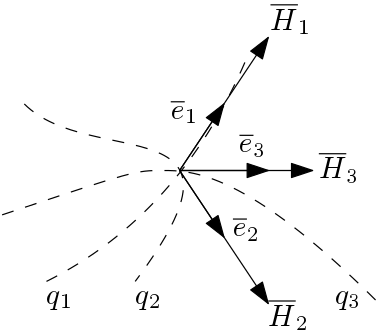
\includegraphics[width=5cm]{fig1.png} 
  \end{figure}  
  
  \begin{gather*}
  \v{r} = \v{r}(q_1(t), q_2(t), q_3(t)) \\
  \v{v} = \dot{\vec {r}}= \sum \limits_{i = 1}^3 \frac{\partial\v{r}}{\partial q_i} \dot q_i\\
  \v{H_i} = \frac{\partial\v{r}}{\partial q_i} = H_i \v{e_i} \text{, где $H_i$ - коэффициенты Ламе.} \\ 
  \end{gather*}
  \subsubsection*{Геометрический смысл}
  $$ ds_i = H_i dq_i $$
  $s_i$ - длина дуги $i$-й координатной линии.
  $$ H_i = \abs{\frac{\partial \v{r}}{\partial q_i}}  = \sqrt{\left(\frac{\partial x}{\partial q_i}\right) ^2 + \left(\frac{\partial y}{\partial q_i}\right) ^2 + \left(\frac{\partial z}{\partial q_i}\right) ^2} $$
  $$ \v{v} = \sum\limits_{i=1}^3 H_i \dot{q_i} \v{e_i},~~ v^2 = (\v{v}, \v{v}) = \sum H_i^2\dot{q_i^2} $$ 
  \begin{teo}
  Компоненты вектора ускорения в ортогональном криволинейном базисе определяются равенством:
  $$ w_i = \frac{1}{H_i}\left(\frac{d}{dt} \frac{\partial}{\partial \dot q_i} \left(\frac{v^2}{2}\right) - \frac{\partial}{\partial q_i} \left(\frac{v^2}{2} \right) \right) $$
  \end{teo}
  \begin{proof}
  \begin{gather*}
(\v{w}, \v{H_i}) = \left(\frac{d\v{v}}{dt}, \frac{\partial \v{r}}{\partial q_i} \right) = \frac{d}{dt} \left(\v{v}, \frac{\partial \v{r}}{\partial q_i}\right) - \left(\v{v}, \frac{d}{dt} \frac{\partial \v{r}}{\partial q_i} \right) \triangleq \\
1) ~ \frac{\partial \v{r}}{\partial q_i} = \frac{\partial \v{v}}{\partial \dot q_i} \text{ - из определения скорости} \\
2) ~ \frac{d}{dt} \left(\frac{\partial \v{r}}{\partial q_i} \right) = \sum \limits_{j = 1}^3 \frac{\partial^2 \v{r}}{\partial q_j \partial q_i} \dot q_j = \sum \limits_{j = 1}^3 \frac{\partial^2 \v{r}}{\partial q_i \partial q_j} \dot q_j = \\ 
= \frac{\partial}{\partial q_i} \left( \frac{d\v{r}}{dt} \right) = \frac{\partial \dot{\vec r}}{\partial q_i} = \frac{\partial \v{v}}{\partial q_i} \\
\triangleq \frac{d}{dt} \left(\v{v}, \frac{\partial \v{v}}{\partial \dot q_i} \right) - \left( \v{v}, \frac{\partial \v{v}}{\partial q_i} \right) = \frac{d}{dt} \frac{1}{2} \frac{\partial}{\partial \dot q_i} (\v{v}, \v{v}) - \frac{1}{2} \frac{\partial}{\partial q_i} (\v{v}, \v{v}) = \\ 
= \frac{d}{dt} \frac{\partial}{\partial \dot q_i} \left(\frac{v^2}{2} \right) - \frac{\partial}{\partial q_i} \left(\frac{v^2}{2}\right) \\
w_i = (\v{w}, \v{e_i}) = \frac{1}{H_i}(\v{w}, \v{H_i})
  \end{gather*}
  \end{proof}